\FloatBarrier
\begin{figure}[H]
\begin{minipage}[b]{0.5\textwidth}

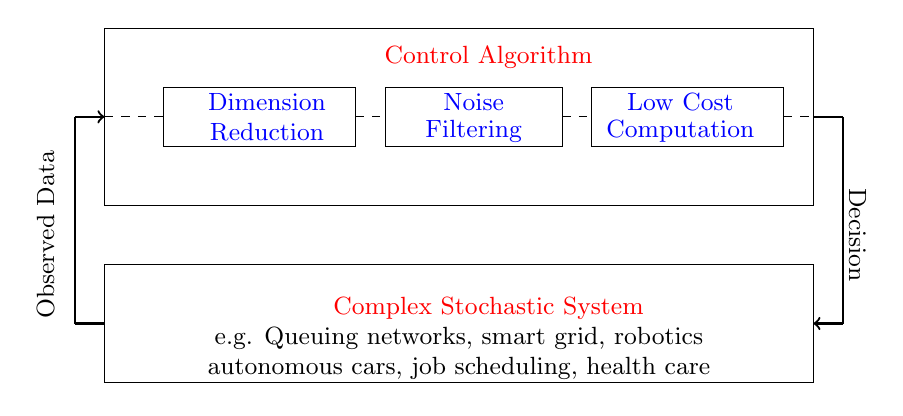
\begin{tikzpicture}[scale=0.75,font=\small,axis/.style={very thick, ->}]
%\draw [black](-2.25,-1) rectangle (2.25,2);
%\node[blue] at(0,1.75) {Modelling};
%\node[blue] at(-1.5,-1.5) {MDP};
%\node[blue] at(-1.5,-1.8) {\&};
%\node[blue] at(-1.5,-2.1) {SMPL};
%\draw[thick,->](-1.5,-1.4)--(-1.5,-0.75);






%\node[blue] at(8,-1.5) {ADP,RL,SPSA};
%\node[blue] at(8,-1.8) {\&};
%\node[blue] at(8,-2.1) {RL};

%\draw[thick,->](8,-1.4)--(8,0.1);
\node[red] at(4.5,4.5) {Control Algorithm};
\draw[black](-2,5) rectangle (10,2);


\draw [black](-1,3) rectangle (2.25,4);
\node[blue] at(.75,3.75) {Dimension};
\node[blue] at(.75,3.25) {Reduction};

\draw [black](5.75,3) rectangle (2.75,4);
\node[blue] at(4.25,3.75) {Noise};
\node[blue] at(4.25,3.25) {Filtering};

\draw [black](6.25,3) rectangle (9.5,4);
\node[blue] at(7.75,3.75) {Low Cost};
\node[blue] at(7.75,3.25) {Computation};

\node[red] at(4.5,0.25) {Complex Stochastic System};
\node[black] at(4,-0.25) {e.g. Queuing networks, smart grid, robotics};
\node[black] at(4,-0.75) {autonomous cars, job scheduling, health care};
\draw[black](-2,1) rectangle (10,-1);

\draw[thick,->](-2.5,3.5)--(-2,3.5);
\draw[thick,-](-2.5,3.5)--(-2.5,0);
\draw[thick,-](-2.5,0)--(-2,0);

\draw[dashed,-](-2,3.5)--(-1,3.5);
\draw[dashed,-](2.25,3.5)--(2.75,3.5);
\draw[dashed,-](5.75,3.5)--(6.25,3.5);
\draw[dashed,-](9.5,3.5)--(10,3.5);

\draw[thick,-](10,3.5)--(10.5,3.5);
\draw[thick,-](10.5,3.5)--(10.5,0);
\draw[thick,->](10.5,0)--(10,0);


\node[rotate=90] at(-3,1.5) {Observed Data};
\node[rotate=270] at(10.75,1.5) {Decision};

\end{tikzpicture}

\end{minipage}
\begin{minipage}[b]{0.5\textwidth}
\centering
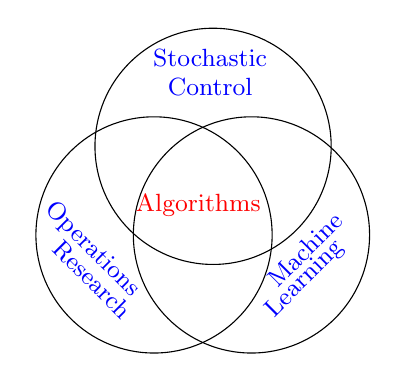
\begin{tikzpicture}[scale=0.75,font=\small,axis/.style={very thick, ->}]
\draw [] (0.9,0.5) circle (2);
\draw [] (-0.75,0.5) circle (2);
\draw [] (.25,2) circle (2);
%\draw [] (-0.5,0.5) circle (2);
%\draw [] (0.5,-0.5) circle (2);
%\draw [] (-0.5,-0.5) circle (2);

\node[red] at(0,1){Algorithms};
%\node[red] at(0,0.5) {Control};
\node[blue,rotate=45] at(1.8,.25){Machine};
\node[blue,rotate=45] at(1.8,-0.25){Learning};

\node[blue,rotate=-45] at(-1.8,.25){Operations};
\node[blue,rotate=-45] at(-1.8,-0.25){Research};

\node[blue] at(0.2,3.5){Stochastic};
\node[blue] at(0.2,3){Control};
\end{tikzpicture}

\end{minipage}


\label{plan}
\captionsetup{font=footnotesize}
\captionof{figure}{On the left is a schematic of a data-driven control algorithm; the observed data is mapped to a decision rule. The challenge is to design control algorithms that are data efficient, computationally cheap and scalable. The right diagram shows the overlap between three areas. Stochastic control has been used to address problems in operations research in the past. A recent trend has been to used machine learning techniques to build data-driven control algorithms.}
\end{figure}
